\chapter{Testes Hipóteses}

Um \textbf{teste de hipóteses} é um procedimento que usa estatística amostral para testar uma alegação sobre o valor de um parâmetro populacional. A finalidade de testes de hipóteses é avaliar uma afirmação sobre os valores de parâmetros populacionais. Uma alegação sobre um parâmetro populacional é chamada de \textbf{hipótese estatística}. Para testar uma hipótese estatística, você deve estabelecer cuidadosamente um par de hipóteses – uma representa uma alegação e a outra, seu complemento.

A \textbf{Hipótese Nula} (denotada por \(H_0\)) é uma hipótese estatística que contém uma
afirmativa de igualdade e deve escrever como \( = , \leq , \geq \). A \textbf{Hipótese Alternativa} (denotada por \(H_a\)) é o complemento da hipótese nula. É uma afirmativa que deve ser verdadeira se \(H_0\) for falsa e contém uma afirmativa de desigualdade, tal como \(<, \neq, ou > \).

A figura \ref{fig:hipoteses-estatisticas} a seguir mostra a relação entre as afirmativas verbais possíveis sobre o parâmetro \(\mu\) e as hipóteses nula e alternativa correspondentes. Afirmativas semelhantes podem ser feitas para outros parâmetros populacionais, tais como p (proporção), \(\sigma\) (desvio padrão) ou \(\sigma^2\) (variância).

\begin{figure}[h]
	\center
	\caption{Hipóteses Estatísticas para \(\mu\)}	
	\label{fig:hipoteses-estatisticas}
	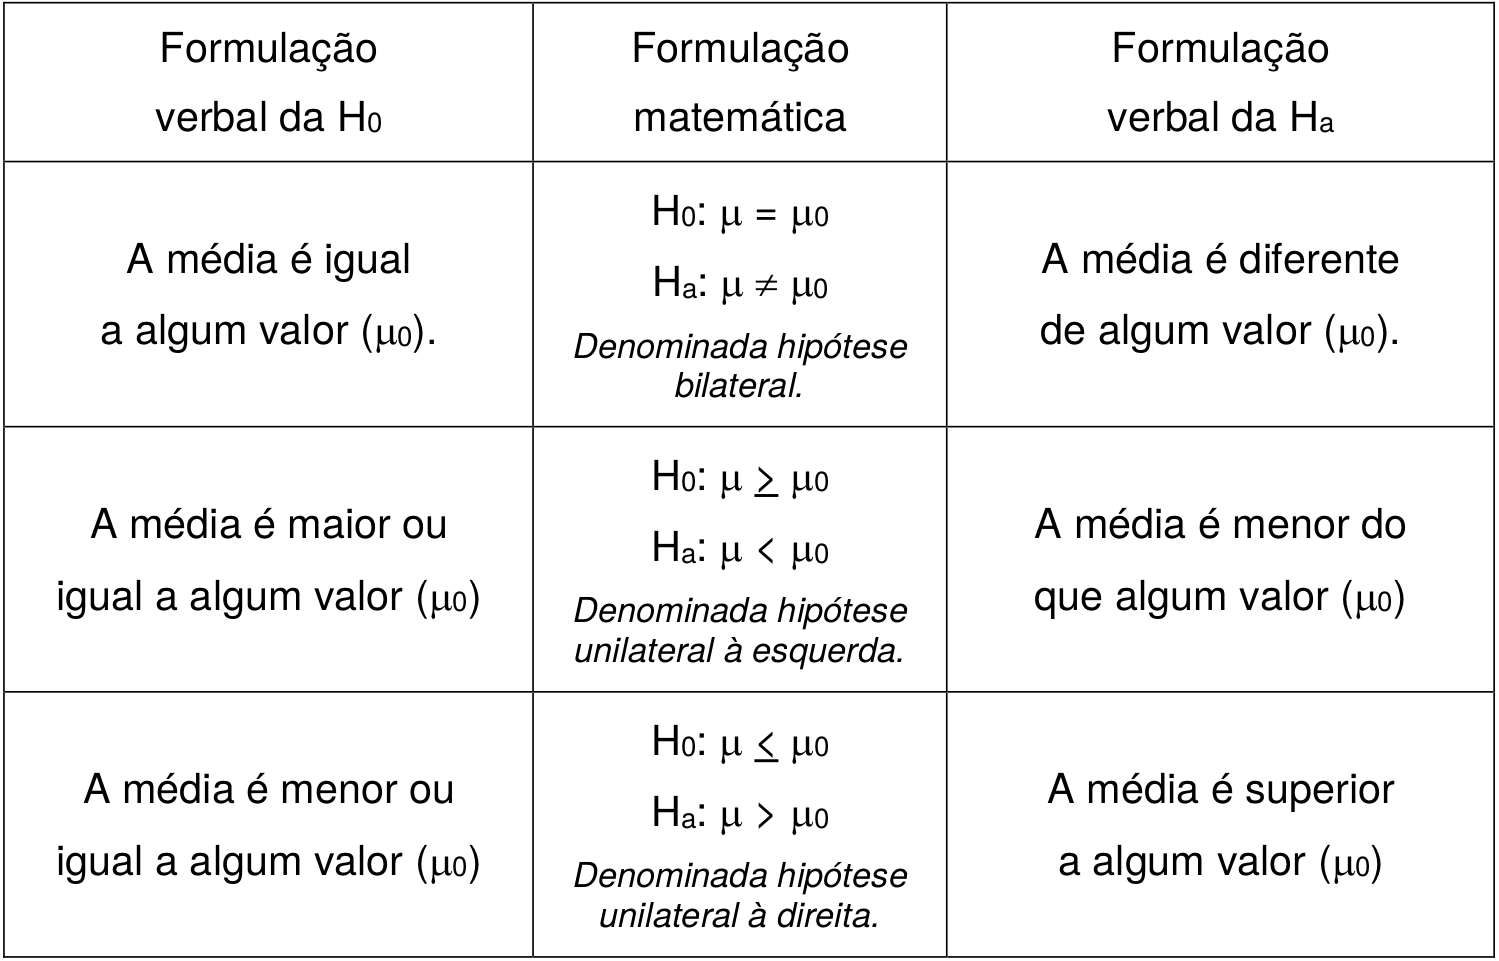
\includegraphics[scale=1.2]{testes-hipoteses/hipoteses-estatisticas.png}
\end{figure}

\section{Tipos de Erro e Nível de Significância}

Não importando qual das hipóteses representa a alegação, você começará sempre um teste de hipóteses assumindo que a condição de igualdade na hipótese nula é verdadeira. Assim, quando realizar um teste de hipóteses, você deve tomar uma de duas decisões: rejeitar a hipótese nula ou aceitar a hipótese nula.

Uma vez que sua decisão baseia-se em informação incompleta (uma amostra em vez de toda a população), há sempre a possibilidade de se tomar a decisão errada. A figura \ref{fig:resultados-teste-hipoteses} mostra os quatro resultados possíveis de um teste de hipóteses.

\begin{figure}[h]
	\center
	\caption{Possíveis Resultados para um Teste de Hipóteses}	
	\label{fig:resultados-teste-hipoteses}
	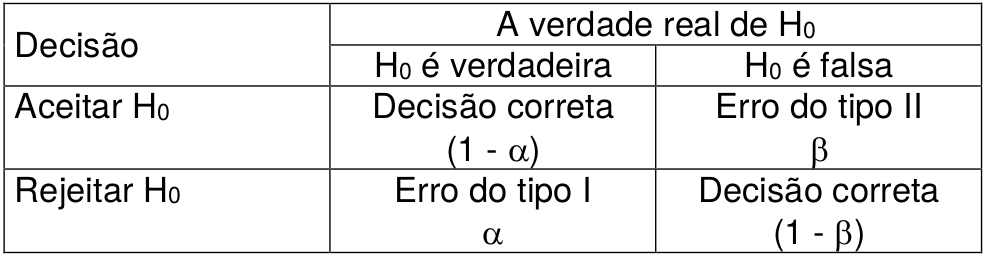
\includegraphics[scale=1.7]{testes-hipoteses/resultados-teste-hipoteses.png}
\end{figure}

O \textbf{nível de significância (\(\alpha\))} de um teste é a probabilidade de uma hipótese nula ser rejeitada, quando verdadeira. Uma das etapas de nosso processo de teste de hipóteses envolve a escolha do nível de significância. Pode-se mostrar, matematicamente, que \(\alpha\), \(\beta\) e o tamanho (n) da amostra estão todos inter-relacionados, de forma que, escolhidos quaisquer dois deles, o terceiro está
automaticamente determinado. Valem as seguintes considerações de ordem prática:
\begin{alineas}
\item Para \(\alpha\) fixo, um aumento do tamanho n da amostra ocasiona uma redução
de \(\beta\); isto é, uma amostra maior reduz a chance de cometermos o erro de aceitar a hipótese nula quando ela é falsa.
\item Para um tamanho n, fixo, de amostra, uma diminuição de \(\alpha\) acarreta um
aumento de \(\beta\); reciprocamente, um aumento de \(\alpha\) acarreta uma diminuição de \(\beta\).
\item Para reduzir \(\alpha\) e \(\beta\), devemos aumentar o tamanho da amostra.
\end{alineas}

\section{Estatística de Teste, Região Crítica e Valor Crítico}

A \textbf{estatística de teste} é uma estatística amostral, ou um valor baseado nos dados
amostrais. Utiliza-se uma estatística de teste para tomar uma decisão sobre a rejeição
ou não da hipótese nula. A \textbf{região crítica} é o conjunto de todos os valores da estatística de teste que levam à rejeição da hipótese nula. O \textbf{valor crítico} é o valor, ou valores, que separa(m) a região crítica dos valores da estatística de teste que não levam à rejeição da hipótese nula. Os valores críticos dependem da natureza da hipótese nula, da distribuição amostral principal, e do nível de significância.

O método clássico de testes de hipóteses  utilizando região crítica constiste nos seguintes passos:
\begin{alineas}
\item Identificar a hipótese nula (contém a condição de igualdade) e a hipótese alternativa (complementar);
\item Escolher o nível de significância com base na gravidade do erro tipo I. São
muito comuns os valores 0,05 e 0,01;
\item Identificar o teste a ser utilizado;
\item Determinar a estatística de teste;
\item Determinar o(s) valor(es) crítico(s) e a região crítica;
\item Rejeitar \(H_0\) se a estatística de teste está na região crítica. Aceitar \(H_0\) se a estatística de teste não está na região crítica;
\item Formular uma conclusão que descreva a conseqüência prática dos dados e dos cálculos.
\end{alineas}

\section{Teste z para uma Amostra (\(\sigma\) conhecido)}

O teste z é utilizado em testes de hipóteses para a média quando valor do desvio padrão (\(\sigma\) é conhecido. Identificadas as hipóteses estatísticas (\(H_0\) e \(H_a\)) e definido o nível de significância (\(\alpha\)), podemos proceder ao cálculo da estatística de teste utilizando a fórmula a seguir.

\[\beq{ z_{teste} = \frac{\hat{x}-\mu_0}{\frac{\sigma}{\sqrt{n}}} } \]

Onde \(\mu_0\) representa o valor da média que está sendo testado, \(\sigma\) representa o desvio padrão populacional, n é o tamanho da amostra e \(\hat{x}\) é a média da amostra.

\subsection{Com base no nível de significância (\(\alpha\))}

\begin{itemize}
	\item Fornecidos: \(\alpha\), \(\mu_0\), \(\hat{x}\) e \(\sigma\)
	\item Aplicar a fórmula de \(z_{teste}\)
	\item Encontrar \(z_{\alpha}\) considerando:
	\begin{itemize}
		\item O sinal de \(z_{teste}\)
		\item O tipo de hipótese (unilateral à esquerda, à direita ou bilateral)
		\item A interpretação da probabilidade na Tabela da Normal Reduzida
	\end{itemize}
\end{itemize}		
	
\subsection{Com base no valor \(p\)}

\begin{itemize}
	\item Fornecidos: \(\alpha\), \(\mu_0\), \(\hat{x}\) e \(\sigma\)
	\item Aplicar a fórmula de \(z_{teste}\)
	\item Encontrar \(p\) considerando:
	\begin{itemize}
		\item O sinal de \(z_{teste}\)
		\item O tipo de hipótese: unilateral à esquerda, à direita ou bilateral 
		\item \(p\) acompanha \(H_a\)
		\item A interpretação da probabilidade na Tabela da Normal Reduzida
		\item Interpretação: comparar \(p\) e \(\alpha\). Se \(p \leq \alpha\) a hipótese nula deve ser rejeitada.
	\end{itemize}
\end{itemize}		

\subsection{Com base no intervalo de confiança}

A correspondência direta entre um intervalo de confiança e um teste de hipótese pode ser feita somente quando o teste é bilateral.

\section{Teste t para uma amostra (\(\sigma\) desconhecido)}

O teste t é utilizado em testes de hipóteses para a média quando valor do desvio padrão (\(\sigma\) é desconhecido. Nesse caso, deve utilizar o desvio padrão amostral (\(s\)) e a distribuição t-Student. Identificadas as hipóteses estatísticas (\(H_0\) e \(H_a\)) e definido o nível de significância (\(\alpha\)), podemos proceder ao cálculo da estatística de teste utilizando a fórmula a seguir.

\[\beq{ t_{teste} = \frac{\hat{x}-\mu_0}{\frac{s}{\sqrt{n}}} } \]

Onde \(\mu_0\) representa o valor da média que está sendo testado, \(s\) representa o desvio padrão amostral, n é o tamanho da amostra e \(\hat{x}\) é a média da amostra.

O valor crítico é obtido na tabela t-Student, a partir do número de graus de liberdade (n -1). Após determinar o número de graus de liberdade (na linha da tabela) e localizar, na coluna, o valor correspondente à área da cauda que se deseja obter, o valor crítico será o valor que corresponde ao cruzamento da linha e da coluna que foram determinados. Lembrando que se um valor crítico está localizado na cauda esquerda, devemos considerá-lo negativo.

\subsection{Com base no valor \(p\)}

\begin{itemize}
	\item Fornecidos: \(\alpha\)\footnote{Lembrar de que \(\alpha\) é uma probabilidade.}, \(\mu_0\), \(\hat{x}\) e \(s\)
	\item Aplicar a fórmula para encontrar o \(t_{teste}\)
	\item Encontrar \(p\) considerando:
	\begin{itemize}
		\item O sinal de \(t_{teste}\)
		\item O tipo de hipótese (unilateral à esquerda, à direita ou bilateral)
		\item A interpretação da probabilidade na Tabela da t-Student:
			\begin{itemize}
				\item Buscar o valor mais próximo do \(t_{teste}\) na linha do grau de liberdade
				\item O valor de \(p\) é o cabeçalho correspondente ao valor encontrado na tabela t-Student
			\end{itemize}
		\item Interpretação: comparar \(p\) e \(\alpha\). Se \(p \leq \alpha\) a hipótese nula deve ser rejeitada.
	\end{itemize}
\end{itemize}

\subsection{Com base no intervalo de confiança}

A correspondência direta entre um intervalo de confiança e um teste de hipótese pode ser feita somente quando o teste é bilateral.